\chapter{KẾT QUẢ NGHIÊN CỨU} \label{sec:chapter_3}
\section{Phương pháp tiếp cận}
\subsection{Hệ thống VLC thực tế}
\begin{figure} [ht]
\centering
\captionsetup{justification=centering}
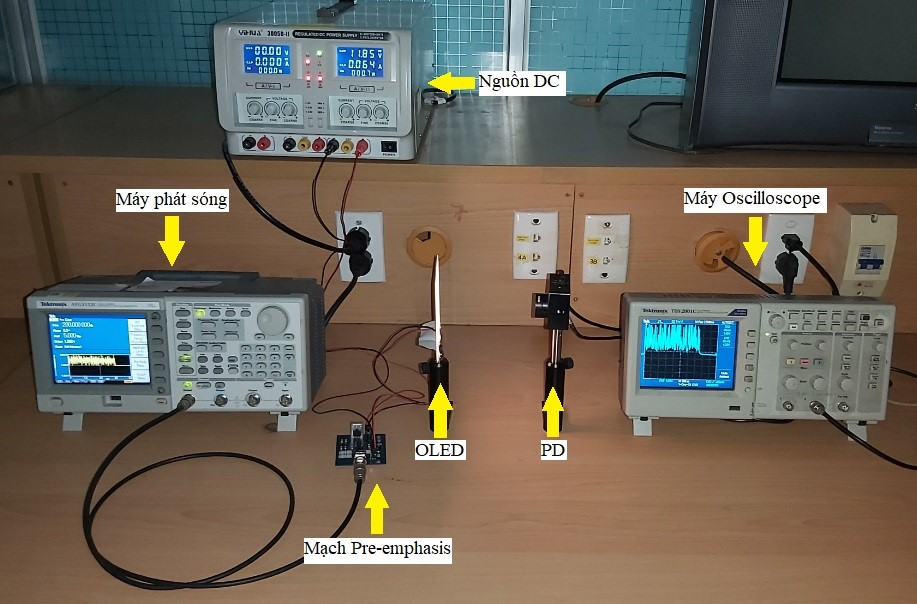
\includegraphics [scale=0.6] {Image/VLC_thucte}
\caption{Hệ thống \ac{vlc} thực tế tại phòng thí nghiệm 209B1}
\end{figure}
\begin{table}[ht]
	\caption{Bảng các thành phần của hệ thống VLC thực tế}.
	\begin{center}
	\small
		\begin{tabular}{|c|c|}
			\hline
			Thiết bị & Thông số\\
			\hline
			\multirow{2}{*}{Generator Tektronik AFG 3152C}
    			&Tốc độ lấy mẫu tối đa 1GS/s, 2 kênh, băng thông 150MHz\\
			&Có thể phát dạng sóng Sine, Square, Pulse, Ramp, Guassian,…. \\			
			&Điều chế AM, FM, PM, FSK, PWM \\
			&Nguồn 100 - 240 V, 47 - 63 Hz\\
			\hline
			\multirow{2}{*}{Oscilloscope Tektronik TDS 2024C}
			&Tốc độ lấy mẫu tối đa 2GS/s\\
			&Băng thông 200MHz\\ 
			&Void/Div tối thiểu 2mV\\
			&4 Channels \\
			\hline
			\multirow{2}{*}{\ac{oled}} \cite{lgN6SA30C} 
			& Băng thông 5KHz\\
			& Kích thước: 100 $\times 100 \times 0.88 mm$\\
			& Công suất tiêu thụ: 1.28 W\\
			& Độ sáng: 75 lm\\
			& Dòng DC: 150 mA\\
			& Điện áp: 8.5 V\\
			\hline
			\multirow{2}{*}{Photodiode (PD)} \cite{APD410A}
			& ADP410A/M của ThorLab \\
			& Bước sóng từ 400 – 1000 nm \\
			& Nguồn: $\pm$ 12 V, 250 mA \\
			\hline
			\multirow{2}{*}{Nguồn DC Yihua 3005D}
			& 0-30 V*2 / 0-5 A*2 \\
			& 2.5 V / 3.3 V / 5 V * 3 A \\
			\hline
		\end{tabular}
		\label{tab:VLC_thucte}
	\end{center}
\end{table}
\paragraph{Điều kiện đo đạc thực tế:}
Hệ thống \ac{vlc} được đặt tại phòng thí nghiệm 209B1, trường Đại học Bách Khoa thành phố Hồ Chí Minh. Nhiệt độ phòng thì nghiệm là $25^o C$, trong điều kiện tắt tất cả các đèn chiếu sáng khác, có ít nguồn sáng tự nhiên từ bên ngoài vào.
\begin{figure}
	\centering
	\begin{subfigure}{.5\textwidth}
		  \centering
		  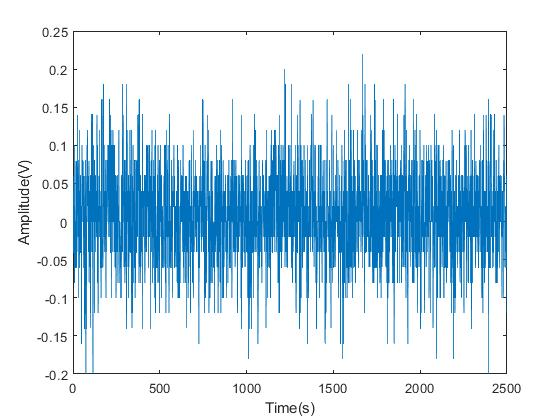
\includegraphics[width=1\linewidth]{Image/floor_noise}
		  \caption{Nhiễu nền trong điều kiện đo đạc của luận văn này}
		  \label{fig: floor_noise}
	\end{subfigure}%
	\begin{subfigure}{.5\textwidth}
		  \centering
		  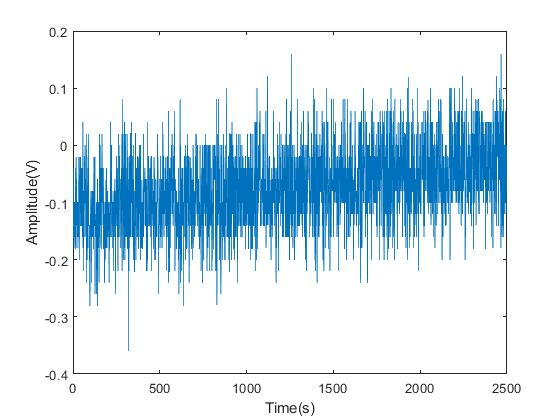
\includegraphics[width=1\linewidth]{Image/fluorescence_noise}
		  \caption{Nhiễu nền trong điều kiện có bật thêm đèn huỳnh quang để chiếu sáng}
		  \label{fig: fluo_noise}
	\end{subfigure}
	\caption{Nhiễu nền trong hai điều kiện}
	\label{fig:noise}
\end{figure}

\begin{figure} [ht]
	\centering
	\captionsetup{justification=centering}
	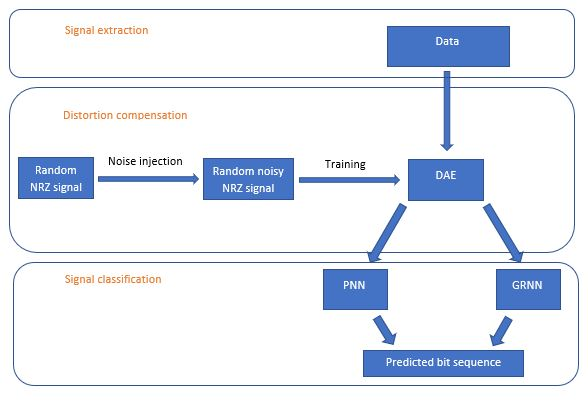
\includegraphics [scale=1] {Image/flow_chart}
	\caption{Sơ đồ khối các phương pháp tiền xử lý và phân loại tín hiệu}
\end{figure}

\subsection{Dữ liệu}
 \paragraph{Tín hiệu phát}
 Để giảm sự thay đổi tín hiệu đột ngột của tín hiệu \ac{nrz}, chúng tôi sử dụng xung Lorentz để thay thế. 
\begin{figure} [ht]
	\centering
	\captionsetup{justification=centering}
	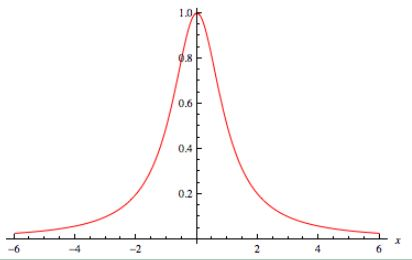
\includegraphics [scale=0.7] {Image/lorentz_pulse}
	\caption{Xung lorentz}
\end{figure}

Hàm Lorentzian với một đỉnh được định nghĩa bởi:

\begin{equation}
L(x) = \frac{1}{\pi}\frac{\frac{1}{2} \Gamma}{{(x-x_0)}^2+ {\frac{1}{2} \Gamma}^2}
\end{equation}
 Trong đó $x_0$ là trung tâm, $\Gamma$ là tham số được đặc trưng bởi chiều rộng có tên là Full Width at Half Maximum. Hàm Lorentz có phân bố xác suất theo phân bố Cauchy. Hàm Lorentz có biến đổi Fourier là 
\begin{equation}
\mathcal{F}[\frac{1}{\pi}\frac{\frac{1}{2}\Gamma}{(x-x_0)^2 + (\frac{1}{2}\Gamma)^2}] =e^{-2\pi i k x_0 - \Gamma \pi |k|.} 
\end{equation}

\paragraph{Trích xuất dữ liệu:}

Tín hiệu truyền đi gồm có 250 ký hiệu, trong đó có 9 ký hiệu pilot dùng để nhận dạng điểm bắt đầu của chuỗi ký hiệu truyền đi. 
Sau khi thu được dữ liệu từ oscilloscope, chuỗi bit truyền đi được trích xuất lại bằng cách so sánh với với chuỗi bit truyền đi thông qua phép tính correlation. 

\begin{figure}
	\centering
	\begin{subfigure}{.5\textwidth}
		  \centering
		  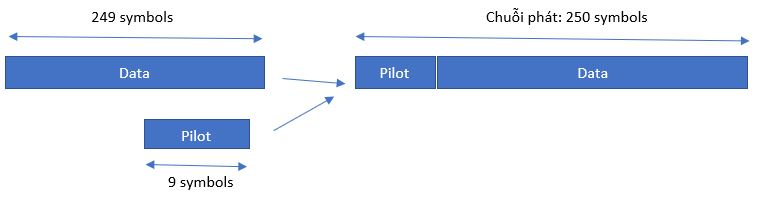
\includegraphics[width=1\linewidth]{Image/data_sequence}
		  \caption{Cấu tạo chuỗi dữ liệu}
	\end{subfigure}%
	\begin{subfigure}{.5\textwidth}
		  \centering
		  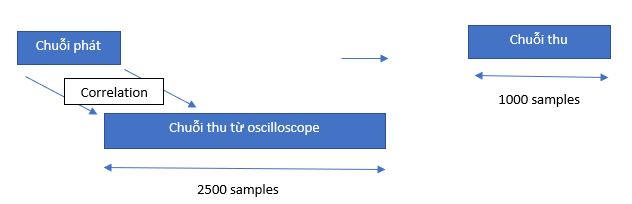
\includegraphics[width=1\linewidth]{Image/data_extracting}
		  \caption{Quá trình trích xuất dữ liệu tại phía thu}
	\end{subfigure}
	\caption{Trích xuất dữ liệu:}
	\label{fig: signal_extraction}
\end{figure}

\paragraph{Phân tích dữ liệu:}

Khi không dùng neural networks, việc giải điều chế sẽ dựa trên một giá trị ngưỡng có thể thay đổi được. Để ước lượng được \ac{snr} của tín hiệu, cần phải tính thông qua giản đồ mắt. Từ giá trị của \ac{snr} có thể tính ra được giá trị của \ac{ber}.

Giá trị \ac{snr} được ước lượng qua công thức:
\begin{equation}
SNR  = \frac {\frac{mean(HighLevel) - mean (LowLevel)}{\sigma(HighLevel) + \sigma(LowLevel)}}{M-1}
\end{equation}
Trong đó: giá trị mức cao và mức thấp được lấy tại thời điểm đồ thị mắt mở rộng nhất. Độ rộng của mắt được tính bằng $(mean(HighLevel) - 3\sigma(HighLevel)) - (mean(LowLevel) + 3\sigma(LowLevel)) $. 

Công thức trên được tính theo Volt, nên cần đổi ra dB bằng cách lấy $20\log_{10}$ kết quả ở trên. 

Có 2 cách để ước lượng \ac{ber} là ước lượng dựa trên \ac{snr} và lấy thương của tổng số bit bị sai và tổng số bit truyền đi. Có thể tính \ac{ber} dựa trên \ac{snr} theo công thức: \cite{Apena_2018}
\begin{equation}
\ac{ber} = \frac{M-1}{M} erfc({\sqrt{\frac{\ac{snr}}{2(M-1)}}})
\end{equation}

\paragraph{Phương pháp đánh giá:} Chất lượng của mô hình được đánh giá thông qua 2 thông số là \ac{snr} và \ac{ber} được tính toán dựa trên 10000 bits thu được (bỏ qua vấn đề đồng bộ ở phía thu và phía phát). Sử dụng kỹ thuật K-fold cross validation để có thể test toàn bộ 10000 bits trên. Dữ liệu được chia ngẫu nhiên thành 5 nhóm, mỗi nhóm 2000 bits, sử dụng 4 nhóm cho việc train và 1 nhóm còn lại cho việc test. Lặp lại cho đến khi test đủ tất cả các nhóm.  

\subsection{Tiền xử lý dữ liệu:}
\paragraph{Framing}
Mỗi symbol đều phụ thuộc vào những symbols đứng trước và sau nó. Vì vậy khi trích dữ liệu để training, chúng ta cần chia dữ liệu thành frame, mỗi frame bao gồm 1 symbol thu được tương ứng với symbol truyền đi cùng với 2 symbols trước và 2 symbols phía sau nó. Như vậy, mỗi frame sẽ bao gồm 5 symbols, các frame liền nhau thì chống lần lên nhau.

\begin{figure} [ht]
	\centering
	\captionsetup{justification=centering}
	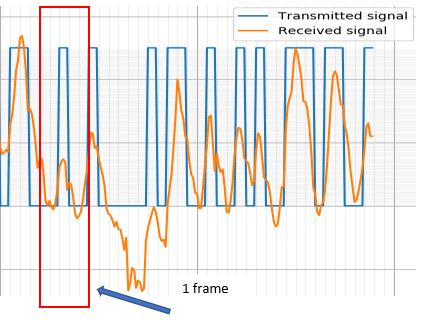
\includegraphics [scale=0.8] {Image/Framing}
	\caption{Cách một frame được trích ra từ tín hiệu thu}
\end{figure}

\paragraph{Đánh giá feature importance bằng Random Forest}
Tại mỗi bit rate, mối quan hệ giữa các symbols và những bit đứng trước và sau nó sẽ có sự khác nhau. Vì vậy, cần một phương pháp có thể đánh giá một cách tương đối mức độ quan trọng của các samples. Trong báo cáo này, chúng tôi sẽ sử dụng Random Forest để đánh giá feature importance.
\begin{figure}
     \centering
     \begin{subfigure}[b]{0.45\textwidth}
         \centering
         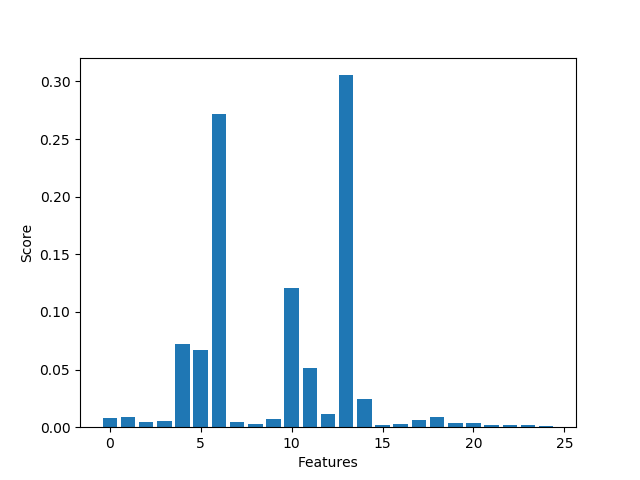
\includegraphics[width=\textwidth]{Image/feature_importance_100k}
         \caption{100kbps}
     \end{subfigure}
     \hfill
     \begin{subfigure}[b]{0.45\textwidth}
         \centering
         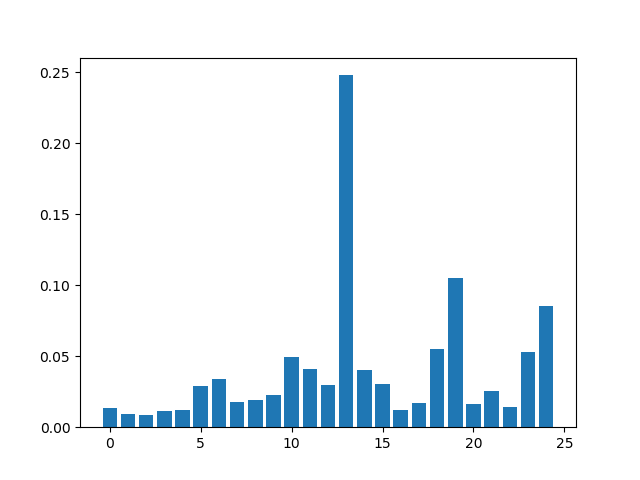
\includegraphics[width=\textwidth]{Image/feature_importance_150k}
         \caption{150kbps}
     \end{subfigure}
     \hfill
     \begin{subfigure}[b]{0.45\textwidth}
         \centering
         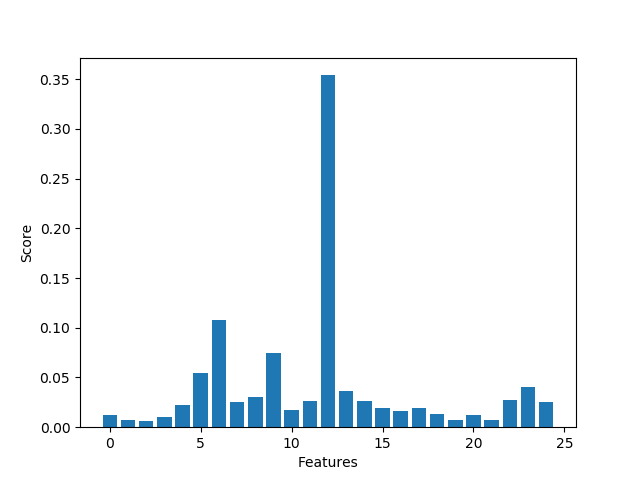
\includegraphics[width=\textwidth]{Image/feature_importance_200k}
         \caption{200kbps}
     \end{subfigure}
          \hfill
     \begin{subfigure}[b]{0.45\textwidth}
         \centering
         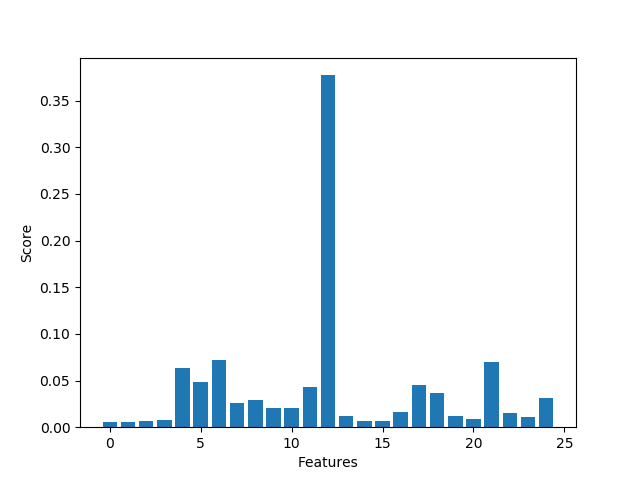
\includegraphics[width=\textwidth]{Image/feature_importance_250k}
         \caption{250kbps}
     \end{subfigure}
        \caption{Đánh giá dữ liệu bằng feature importance}
        \label{fig:feature_importance}
\end{figure}
\paragraph{Áp dụng biến đổi wavelet liên tục}
Mother wavelet được chọn là Mexican hat (richer) vì nó có sự tương đồng nhiều nhất với tín hiệu.
\begin{equation}
\psi(t) = \frac{2}{\sqrt{3} \sqrt[4]{\pi}} \exp^{-\frac{t^2}{2}} \left( 1 - t^2 \right)
\end{equation}
Bề rộng (width) được chọn là 3.
\ac{cwt} chỉ cho kết quả rõ ràng khi tín hiệu có nhiều thông tin hơn. Vì vậy, trong báo cáo này, chúng tôi chỉ áp dụng \ac{cwt} cho trường hợp tín hiệu trước đó đã được tiền xử lý bằng cách lấy theo frame.

\paragraph{Hiệu chỉnh tín hiệu bằng \ac{dae}:}

Như đã trình bày ở chương trước, với giới hạn băng thông điều chế của \ac{oled}, chúng ta phải sử dụng thêm bộ pre-emphasis để làm tăng băng thông. Nhưng cũng chính vì điều này mà méo dạng phi tuyến cũng tăng theo. 
Trong báo cáo này, chúng ta sẽ tập trung vào việc làm giảm sự méo dạng phi tuyến của \ac{oled} bằng bộ bù post-distortion. 

Ngõ vào của mô hình là tín hiệu cùng loại với tín hiệu trước khi qua kênh truyền \ac{vlc}. Mô hình sẽ học theo kiểu unsupervised learning, nghĩa là chỉ học những đặc tính của tín hiệu trước khi qua kênh truyền mà không cần phải dán nhãn. Tín hiệu sử dụng trong hệ thống \ac{vlc} rất đơn giản nên việc bị overfitting là không thể tránh khỏi. Để giảm thiểu overfitting có thể sử dụng kỹ thuật noise injection để tăng độ phức tạm cho dữ liệu đầu vào. 

Để tạo ra dữ liệu để train cho mô hình \ac{dae}, chúng ta cần tạo ra một chuỗi tín hiệu ngẫu nhiên có số lượng mẫu bằng với dữ liệu cần hiệu chỉnh. Ví tín hiệu tạo ra được rất đơn giản nên mô hình sẽ rất dễ bị overfitting, để giảm thiểu tình trạng này, cần áp dụng kỹ thuật noise injection để tăng độ phức tạp cho tín hiệu.

Như vậy, mô hình \ac{dae} sẽ sử dụng tín hiệu sau khi thêm nhiễu để học mà không cần dán nhãn cho tín hiệu. Mô hình sẽ học những đặc trưng của tín hiệu 2 mức khi không bị méo dạng. 
Sau khi mô hình \ac{dae} được training xong, tín hiệu ngõ ra của hệ thống \ac{vlc} sẽ được đưa vào để có thể hiệu chỉnh lại tín hiệu bị méo dạng. (Vì nhiễu là ngẫu nhiên nên chất lượng của mô hình qua mỗi lần train sẽ cho kết quả có đôi chút khác biệt).

Để tăng hiệu quả cho mô hình \ac{dae}, chúng tôi xây dựng các layer dựa trên mô hình \ac{lstm}. \ac{lstm} sẽ giúp mô hình \ac{dae} có thể học được những đặc điểm, mối quan hệ của những bit liền kề. (trong báo cáo này, chúng tôi sẽ không đề cập về cơ sở lý thuyết \ac{lstm}).
Một số thông số cho mô hình \ac{dae} như:
\begin{itemize}
\item Optimizer: Stochastic Gradient Descent with mini batch
\item Learning rate: 0.001
\item Epoch: 100
\end{itemize}

\begin{figure}
	\centering
	\begin{subfigure}{.45\textwidth}
		  \centering
		  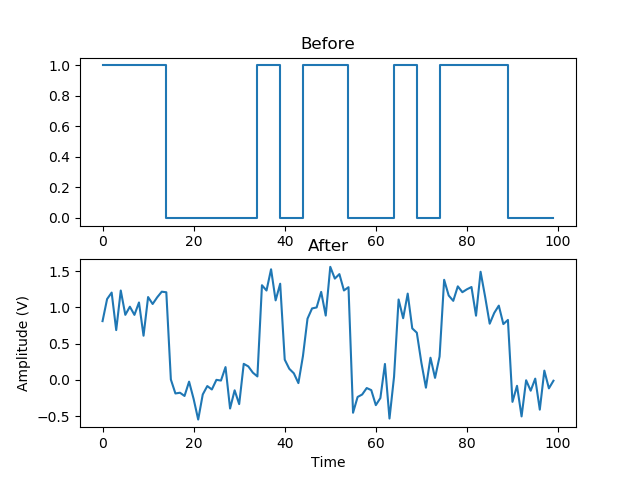
\includegraphics[width=1\linewidth]{Image/dae_noise_injection}
		  \caption{Tín hiệu trước và sau khi thêm nhiễu (dùng cho training)}
		  \label{fig: floor_noise}
	\end{subfigure}
	\begin{subfigure}{.45\textwidth}
		  \centering
		  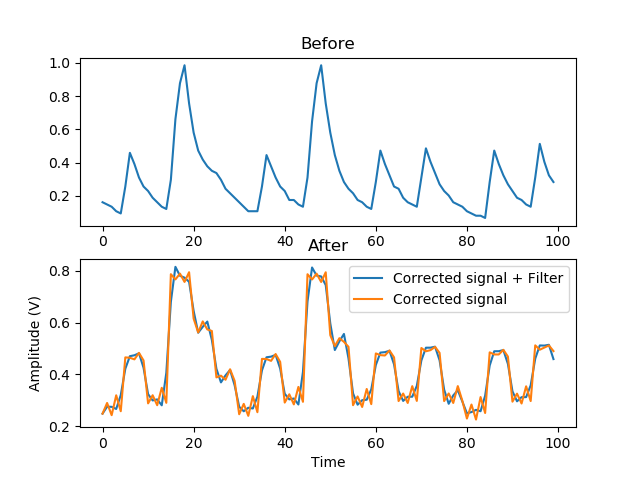
\includegraphics[width=1\linewidth]{Image/corrected_signal}
		  \caption{Tín hiệu ngõ ra của hệ thống \ac{vlc} trước và sau khi được hiệu chỉnh}
		  \label{fig: fluo_noise}
	\end{subfigure}
	\caption{Mô hình \ac{dae}}
	\label{fig:dae}
\end{figure}

Tín hiệu sau khi đi qua mô hình \ac{dae} sẽ có khá nhiều nhiễu, vì vậy nó cần được đi qua thêm một bộ lọc để giảm bớt nhiễu. Có thể thấy tín hiệu sau khi đi qua \ac{dae} và bộ lọc có chất lượng tốt hơn nhiều so với tín hiệu ban đầu. Các mức của tín hiệu có thể dể dàng phân biệt được, như vậy là đã làm giảm đáng kể tình trạng méo dạng của tín hiệu.

\section{Kết quả và phân tích}
\subsection{Khảo sát tín hiệu:} 
Trong phần này, chúng tôi sẽ tiến hành khảo sát tín hiệu tại các tốc độ bit khác nhau để tìm ra tốc độ bit phù hợp để phân tích và so sánh tín hiệu \ac{nrz} với tín hiệu xung Lorentz. Để thấy hiệu quả của các phương pháp tiền xử lý, phân loại cũng như việc sử dụng xung Lorentz, chúng tôi sẽ so sánh các phương pháp này với nhau và với kết quả của những nghiên cứu trước đó cũng tại trường đại học Bách Khoa TP. HCM với cùng một hệ thống \ac{vlc}. Trong đó, sử dụng điều chế \ac{nrz} 2 mức, phân loại bằng \ac{pnn}, không qua tiền xử lý. Tốc độ tối đa đạt được là 25kbps khi ước lượng \ac{ber} thông qua \ac{snr} và 53kbps khi dùng \ac{pnn} để phân loại.

Để thấy hiệu quả của các phương pháp tiền xử lý, phân loại cũng như việc sử dụng xung Lorentz, chúng tôi sẽ so sánh các phương pháp này với nhau và với kết quả của những nghiên cứu trước đó cũng tại trường đại học Bách Khoa TP. HCM với cùng một hệ thống \ac{vlc}. Trong đó, sử dụng điều chế \ac{nrz} 2 mức, phân loại bằng \ac{pnn}, không qua tiền xử lý. Tốc độ tối đa đạt được là 25kbps khi ước lượng \ac{ber} thông qua \ac{snr} và 53kbps khi dùng \ac{pnn} để phân loại (không qua tiền xử lý).

\begin{figure} [ht]
	\centering
	\captionsetup{justification=centering}
	\includegraphics [scale=0.8] {Image/BER_20cm}
	\caption{\ac{ber} ước lượng tại các tốc độ bit khác nhau khi dùng xung Lorentz}
	\label{fig:BER_20cm}
\end{figure}
Hình \ref{fig:BER_20cm} cho thấy, nhìn chung việc dùng tín hiệu xung Lorentz ngõ vào làm cho tín hiệu ngõ ra khó nhận dạng hơn bằng cách ước lượng \ac{ber} thông qua \ac{snr}, không có tốc độ bit nào đạt ngưỡng khi dùng Lorentz. Tuy nhiên nó lại giúp mạch đáp ứng tốt hơn, vẫn có thể phân biệt bằng mắt khi tốc độ vượt quá 70kbps, trong khi đó tín hiệu \ac{nrz} thì không còn phân biệt được nữa.
 
\subsection{Phân loại các mức tín hiệu:}

Hai mô hình được sử dụng trong báo cáo này là \ac{pnn} và \ac{grnn}, cả hai mô hình trên đều được phát triển bởi Specht và đều là mô hình one-pass. Với lợi thế là về mặt tốc độ cũng như khả năng chống chịu nhiễu. Để thể hiện được hiệu quả của 2 mô hình trên, chúng tôi sẽ về \ac{ber} và thời gian (thực hiện trên Google Colab).

Độ lệch chuẩn được chọn cho phương pháp \ac{pnn} khi chỉ lấy một symbol khá nhỏ (từ 0.05 đến 0.3) và tăng dần khi tăng khoảng cách. Đối với \ac{grnn}, độ lệch chuẩn lớn hơn nhiều lần so với \ac{pnn} (từ 3 đến 7), và cần giảm dần khi tăng khoảng cách. Đối với trường hợp sử dụng \ac{dae}, độ lệch chuẩn cần nhỏ hơn từ 5 đến 10 lần với \ac{pnn} và lớn hơn từ 5 đến 10 lần với \ac{grnn}.

\begin{table}[ht]
	\caption{Bảng so sánh độ chính xác của các phương pháp khi chỉ lấy một symbol}.
	\begin{center}
	\small
		\begin{tabular}{|c|c|c|c|c|}
			\hline 
			\backslashbox{Phương pháp}{Khoảng cách(cm) } & 10& 20 & 30 & 40\\
			\hline
			Không dùng neural networks & 0.1928 & 0.2077 & 0.2006 & 0.2194\\
			\hline 
			\ac{pnn} & 0.1377 & 0.1867 & 0.1744 & 0.2089\\
			\hline
			\ac{grnn} & 0.1394 & 0.1861 & 0.1745 & 0.2090\\
			\hline
			\ac{pnn} + \ac{dae} & 0.0356 & 0.0544 & 0.0585 & 0.0999\\
			\hline
			\ac{grnn} + \ac{dae} & 0.0347 & 0.0053 & 0.0566 & 0.0910\\
			\hline
		\end{tabular}
		\label{tab:result_1}
	\end{center}
\end{table}

Khi lấy dữ liệu theo frame và áp dụng \ac{cwt}, cần chọn độ lệch chuẩn trong hai phương pháp là \ac{pnn} và \ac{grnn} cao hơn so với không dùng \ac{cwt}, thông thường là gấp đôi.
\begin{table}[ht]
	\caption{Bảng so sánh độ chính xác của các phương pháp khi lấy một frame}.
	\begin{center}
	\small
		\begin{tabular}{|c|c|c|c|c|}
			\hline 
			\backslashbox{Phương pháp}{Khoảng cách(cm) } & 10& 20 & 30 &40\\
			\hline
			\ac{pnn} & 0.0065 & 0.0096 & 0.0125 & 0.0321\\
			\hline
			\ac{grnn} & 0.0064 & 0.0095 & 0.0127 & 0.0311\\
			\hline
			\ac{pnn} + \ac{cwt} & 0.0065 & 0.0085 & 0.0118 & 0.0341\\
			\hline
			\ac{grnn} + \ac{cwt} & 0.0067 & 0.0088 & 0.0119 & 0.0338\\
			\hline 
			\ac{dtnn} & 0.0052 & 0.0087 & 0.0126 & 0.0317\\
			\hline
		\end{tabular}
		\label{tab:result_2}
	\end{center}
\end{table}

Từ kết quả thu được như trên, có thể thấy việc dùng \ac{dae} để bù méo dạng đem lại hiệu quả tốt nhất khi chỉ dùng một symbol để phân loại. Trong khi đó, framing mang lại hiệu quả đáng kể cho việc nhận dạng. Từ đó, ý tưởng của chúng tôi là kết hợp hai loại dữ liệu này lại với nhau và mô hình \ac{dtnn} là lựa chọn vô cùng phù hợp trong trường hợp này.

\begin{table}[ht]
	\caption{Bảng so sánh thời gian train và test các phương pháp}
	\begin{center}
	\small
		\begin{tabular}{|c|c|c|c|}
			\hline 
			Phương pháp & Thời gian train (s) & Thời gian test (s)\\
			\hline 
			\ac{pnn} & - & 4.63 \\
			\hline
			\ac{grnn} & - & 19.53\\
			\hline
			\ac{dae} & 103.25 & 1.9291 \\
			\hline
			\ac{pnn} + Framing & - & 12.18 \\
			\hline
			\ac{grnn} + Framing & - & 35.11 \\
			\hline
			\ac{pnn} + \ac{cwt} & - & 47.37 \\
			\hline
			\ac{grnn} + \ac{cwt} & - & 86.22 \\
			\hline
			\ac{dtnn} & - & 63.51 \\
			\hline
		\end{tabular}
		\label{tab:time}
	\end{center}
\end{table}
Thời gian train và test của các phương pháp được thể hiện trong bảng \ref{tab:time}, trong đó kết quả test trên Google Colab. Chỉ có mô hình \ac{dae} là có thể lưu lại mô hình và sử dụng cho nhiều bit rate và khoảng cách khác nhau. Vì sử dụng K-fold validation để đánh giá dữ liệu nên không thể lưu lại mô hình cho \ac{dtnn} mà phải train lại cho mỗi lần cần test. Trong trường hợp có đủ dữ liệu (lớn hơn 20000 bits), có thể lưu lại mô hình \ac{dtnn}, từ đó thời gian test có thể giảm đi khoảng 3-4 lần. 

\section{Kết luận chương}
Trong báo cáo này, chúng tôi đã xây dựng các mô hình có khả năng phân loại các mức tín hiệu và các mô hình để tiền xử lý cho tín hiệu. Để thấy được sự hiệu quả, chúng tôi đã so sánh các phương pháp này với nhau và với kết quả từ nghiên cứu trước đó.

Đầu tiên, chúng ta sẽ đi so sánh các phương pháp tiền xử lý tín hiệu. Từ bảng \ref{tab:result_1} có thể thấy việc phân loại tín hiệu bằng neural networks (không qua tiền xử lý) vẫn đem lại hiệu quả đôi chút so với khi không dùng. Tuy nhiên sai số vẫn còn rất lớn và không thể ứng dụng cho mô hình thực tế. Sau đó, sau khi dùng thêm \ac{dae} để hiệu chỉnh tín hiệu \ac{ber} đã giảm đáng kể, giảm 4 lần. Mặc dù vậy, \ac{ber} vẫn còn khá cao, chưa thể áp dụng vào hệ thống \ac{vlc} được. Việc hiệu quả của \ac{dae} chưa cao như kỳ vọng là do ngay từ đầu tín hiệu truyền đi không phải là xung vuông, trong khi đó nhiệm vụ của \ac{dae} là đưa tín hiệu về càng giống tín hiệu \ac{nrz} càng tốt.

Nhận thấy các bit liền kề có sự liên hệ với nhau, chúng tôi đã ứng dụng một kỹ thuật của xử lý tiếng nói là Framing để tăng độ chính xác cho mô hình. Từ bảng \ref{tab:result_2}, có thể thấy Framing giúp \ac{ber} giảm đi 20 lần xuống dưới mức 0.01 tại các khoảng cách 10 và 20 cm. Ngoài ra, chúng tôi còn áp dụng thêm một kỹ thuật khác là \ac{cwt}, kết quả cho thấy \ac{ber} giảm đi đôi chút. Từ kết quả của Framing và \ac{dae}, chúng tôi đã sử dụng \ac{dtnn} để giảm \ac{ber}, kết quả là \ac{dtnn} cũng giúp giảm \ac{ber}, đặc biệt là ở 10 cm.

Kế đến, chúng tôi sẽ so sánh 3 phương pháp được sử dụng trong luận văn là \ac{pnn}, \ac{grnn} và \ac{dtnn}. Từ ba bảng \ref{tab:result_1}, \ref{tab:result_2} và \ref{tab:time} cho thấy \ac{pnn} và \ac{grnn} mang lại hiệu quả tương đối ngang nhau, \ac{dtnn} thì nhỉnh hơn đôi chút. Tuy nhiên, thời gian chính là ưu thế rất lớn của \ac{pnn} so với hai phương pháp còn lại. Ngoài ra, xét về tính khả thi khi triển khai mô hình thực tế, \ac{pnn} và \ac{grnn} cũng chiếm phần lợi thế hơn so với \ac{dtnn} vì chỉ sử dụng các phép tính toàn đơn giản, hoàn toàn có thể lập trình bằng C/C++ trên những vi xử lý giá rẻ, không cần lập trình Python trên các vi xử lý đắt tiền hơn như \ac{dtnn}.

Tóm lại, qua khảo sát ở trên có thể thấy xung Lorentz làm tín hiệu trở nên khó phân loại hơn so với \ac{nrz}. Tuy nhiên, nó lại giúp mạch đáp ứng tốt hơn. Từ đó, khi kết hợp Lorentz cùng với những phương pháp mạnh mẽ hơn có thể mang lại hiệu quả đáng kể. Khảo sát của chúng tôi cho thấy, phương pháp của chúng tôi có thể giúp bit rate tăng 4 lần so với phương pháp truyền thống và tăng gần 2 lần so với khi áp dụng tín hiệu \ac{nrz} cùng với những phương pháp xử lý đơn giản.